% CREATED BY DAVID FRISK, 2016
\chapter{Methods}
\todo{REWRITE TO PAST TENSE}
I am working with AI Habitat, a simulation platform for working with embodied AI\cite{habitat19iccv}. It consists of two parts, Habitat-Sim, the 3D simulator, and Habitat-Lab, the library for embodied AI development. 

\subsection{The Model}
I am starting with the Embodied Question Answering baseline in Habitat-Lab, which consists of three parts, a CNN for initial feature extraction, a question answering module, and a navigation module, called PACMAN\cite{embodiedqa}.
The CNN feature extractor is trained on three tasks: RGB reconstruction, semantic segmentation, and depth estimation.
The question answering module is given the last five frames of navigation (in training taken during ground-truth shortest path navigation), and then predicts an answer from a set of possible answers. 
The navigation is trained via imitation learning to imitate shortest path navigation. \todo{Maybe include an example of the json for an episode?} 
The training of the Habitat-Lab version of the model differs somewhat to the version presented in the Embodied Question Answering paper. For the original model, the CNN, question answering, and navigation modules were all trained separately, and then reinforcement learning was used to fine-tune, and more strongly link the question answering and navigation modules, by using accurate question answering as part of the reward for the navigation module. This reinforcement learning is missing from the habitat version of the model; the components of the model are only trained separately. 

\section{The Datasets}
\todo{REWRITE TO PAST TENSE}
I am using the Matterport3D dataset, a dataset of real interiors with human annotation of objects, as my scene dataset\cite{matterport}. 
I am using the MP3D-EQA task dataset, which was created using code to automatically generate questions and answers to correspond with annotated scenes in the Matterport3D dataset\cite{eqa_matterport}. 
\subsection{Interiors}

\subsection{MP3D-EQA Dataset} 
This dataset contains questions of three types: 'color\_room': \emph{What color is the <obj> in the <room>?}, 'color': \emph{What color is the <obj>?}, and 'location': \emph{What room is the <obj> located in?}. \todo{add details about dataset creation} This dataset was based off of the EQA-V1 dataset\cite{embodiedqa}. There were some differences between the datasets, however. The EQA-V1 dataset included a fourth type of question, prepositional questions: \emph{What is <on/above/below/next to? the <obj> in the <room>?}, but these are not present in MP3D-EQA, due to limited occurence of these relationships in the Matterport3D dataset. EQA-V1 was built based on the SUNCG dataset, which is no longer available. 
The paper which introduces the MP3D-EQA dataset was mainly focused on the navigation aspect of the task, and the question types reflect that. A color or location question should theoretically be a good indication of whether or not the agent has successfully navigated to the object, but actually answering the question may not require as complex of reasoning. \todo{discussion of difficulty of color recognition}

\begin{table}[h]
\centering
\caption{Question Type Breakdown}
\begin{tabular}{ |l|l|l| }
\hline
\textbf{question type} & \textbf{percentage of training set} & \textbf{percentage of evaluation set} \\
\hline
color\_room & 69.85908 & 68.46154\\
color & 15.91858 & 17.69231\\
location & 14.22234 & 13.84615\\
\hline
\end{tabular}
\label{tab:q_breakdown}
\end{table}

The dataset has a fixed train/eval split. There is one object which only occurs in the validation set ('toaster'), and one answer that only occurs in the validation set ('gym'). 

\section{Experiment 1: Baseline and Blindfolding}
\label{sec:exp_1}
In this task, I trained and evaluated my baseline model, the CNN and VQA portions of the EQA baseline in habitat-lab. A diagram of the VQA model can be seen in Fig.~\ref{fig:baseline_model}. I also conducted a blindfolding test, in which during evaluation the model was given zeroes instead of the visual information for the scene. This was done by duplicating and modifying the method that converts the .jpgs into numpy arrays to be input to the model, so that it produced an array of zeroes of the same size instead. The point of this blindfolding was to determine if the VQA model was considering the visual input when answering the questions. 

\begin{figure}[h]
     \centering
     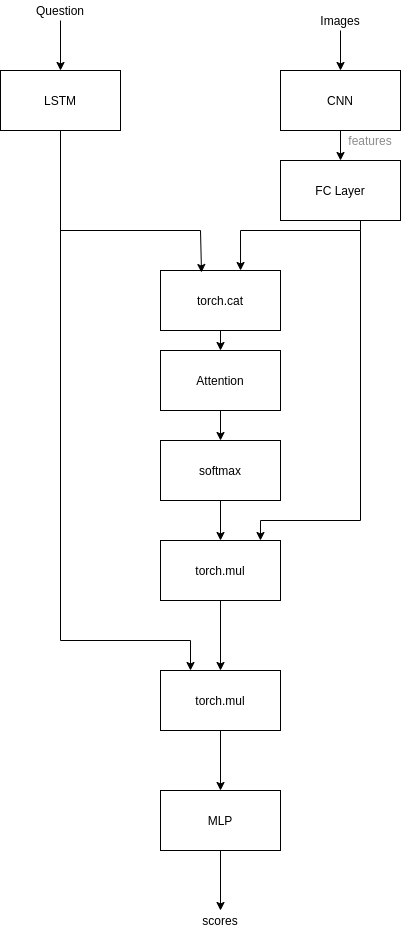
\includegraphics[width=.5\textwidth]{/home/yasmeen/Desktop/thesisproj/thesis/figure/baseline_diagram.png}
     \caption{VQA Model}
     \label{fig:baseline_model}
\end{figure}

\section{Experiment 2: Basic Semantic Categories}
\label{sec:exp_2}
The agent in habitat-sim includes a 'semantic sensor', that reads annotations from the dataset. It reads annotations of object instances, which can then be mapped to category ids. The list of category IDs can be found in appendix~\ref{app:categories}. These category IDs were used as another information source for the model, as shown in Fig.~\ref{fig:category_model}.

\todo{Give more detail on shaping, add motivation}
\begin{figure}[h]
     \centering
     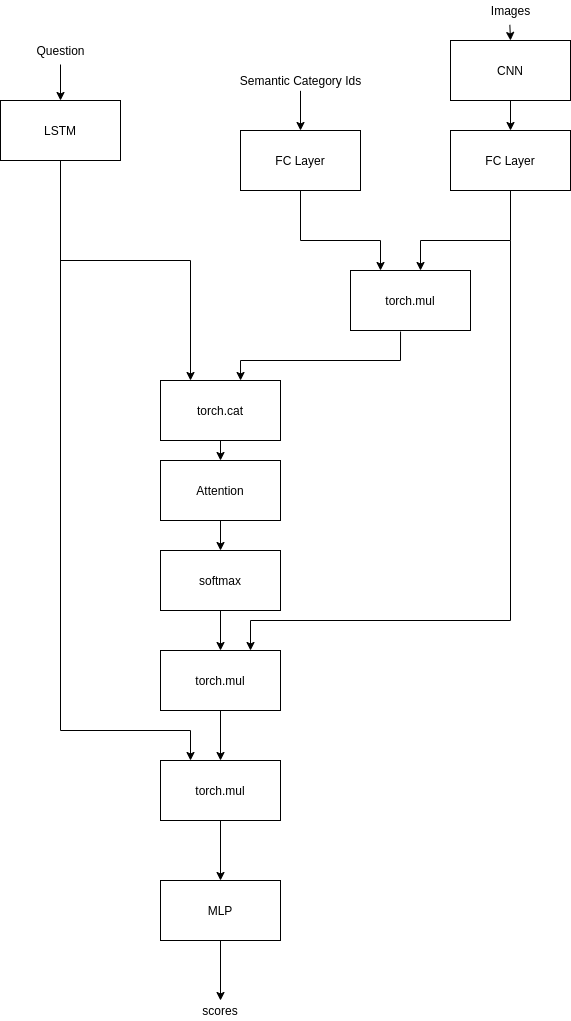
\includegraphics[width=.5\textwidth]{/home/yasmeen/Desktop/thesisproj/thesis/figure/model_w_semantic.png}
     \caption{Model With Semantic Category IDs as 3rd input}
     \label{fig:category_model}
\end{figure}

\section{Experiment 3: DenseCap}
\subsection{Using DenseCap Features}

\subsection{Using DenseCap Boxes}
